%%%%%%%%%%%%%%%%%%%%%%%%%%%%%%%%%%%%%%%%%
% University Assignment Title Page 
% LaTeX Template
% Version 1.0 (27/12/12)
%
% This template has been downloaded from:
% http://www.LaTeXTemplates.com
%
% Original author:
% WikiBooks (http://en.wikibooks.org/wiki/LaTeX/Title_Creation)
%
% License:
% CC BY-NC-SA 3.0 (http://creativecommons.org/licenses/by-nc-sa/3.0/)
% 
% Modified for COSC343 by:
% Lech Szymanski (5/5/2020)
%
% Adapted for AIML402 by:
% Lech Szymanski (18/7/2022)


\documentclass[12pt]{article}
\usepackage{cosc343style}


% Paper code -- change it to AIML402 if you're enrolled in AIML402
\papercode{COSC343}

% Your project title (change appropriately for the assignment)
\title{Assignment 2 report}

% Your name
\author{Kurt \textsc{Wedding-Speight}}
\studentid{6548936}


% Date, change the \today to a set date if you want to be precise
\reportdate{\today}

\begin{document}


\maketitle

\section{Introduction}

This assignment uses a set of code created to make a game very similar to the very old game from 1997 coming from phones, Snake. This implementation of the game includes multiple snakes in the level, though, which differs from the original game where there is only 1 snake.

The purpose of this assignment is to create and develop a Genetic Algorithm capable of evolution. This will be achieved by creating ``sentient" snakes that begin making poor decisions on where to travel on the game field, but evolve to be better through breeding of the more fit snakes in order to make more fit children, and training of the generations to improve future generations.

\section{How the snake functions}

\subsection{Initial Approach and Planning}

My initial approach to this assessment was to create an array of ``random'' chromosomes, each of which representing a snake's decision making.

Then, using that array of chromosomes, each snake can have a unique, possibly good or possibly bad set of values to play the game with.

Once the snakes have their chromosomes, they then recieve data about their immediate surroundings, and use that data to make a decision on where to move.

The creation of the chromosomes was initially done by creating a 3 x nPercepts + 1 array of random values between -1 and 1, but was later changed to be between -20 and 20 iin order to give the snakes more variation in their chromosomes.

\subsection{Altering the Snake's View}
The data given to the snakes about their surroundings needs to be altered before a decision on the movement is made, though.

The percepts given to the agentFunction needs to be changed so that the snakes own body and friendlies are seen as places the snake wants to avoid moving to, as it would be killed.

The influence that fruit have on the snake also needs to be changed to encourage the snake to move to spaces with fruit on them, rather than empty spaces.

I did this by changing all the friendly values from 1 to -20, all enemy values from -1 to -20, and all fruit from 2 to 20

\subsection{Deciding Actions}

In order for each snake to decide the direction it travels in: left, right, or up, the AgentFunction needs to weigh its options and decide based on its chromosome values, in order to create diversity in choice between the snakes.

The way I implemented the weighing up of the actions was by using the following formula to find $a_1$, $a_2$, and $a_3$:

      \[a_1 = w_1p_1 + w_2p_2 + \ldots + w_9p_9 + w_{10}\] 
      \[a_2 = w_{10}p_1 + w_2p_2 + \ldots + w_{19}p_9 + w_{20}\]
      \[a_3 = w_{20}p_1 + w_2p_2 + \ldots + w_{29}p_9 + w_{30}\] \newline
Where $w_n$ is each individual snake chromosome value, and $p_n$ is the value provided to the AgentFunction from the percepts, the snakes immediate vicinity information.

The values $a_1$, $a_2$, and $a_3$ are then compared to each other, and the index of the highest value is chosen and returned for the snake to make its movement decision.

\subsection{Evaluating Snake Fitness}

In order to measure whether a snake performed well, or did not perform well, I initially used a fitness function that rewards snakes for collecting ``fruit'', and staying alive longer.

This initial fitness function can be described as:
      
      \[fitness = fruitCollected + \frac{turnsAlive}{maxTurns}\]

An issue I ran into with this fitness function was that it encourages staying alive, so snakes can evolve to spin in circles where they are completely safe instead of targeting fruit in order to grow.

This is not what I wanted the snakes to do, so I altered the equation, making the $turnsAlive$ variable worth less towards the snake fitness. 

After finding this, I changed the fitness function to be:

      \[fitness = fruitCollected + \frac{turnsAlive}{2*maxTurns}\]
      
\subsection{Breeding of New Snakes}

Once the fitness of each snake is found, the snakes need to ``breed'' to create a new, hopefully evolving generation.

In order to implement the breeding, I tested 2 different methods, and compared which produced better children.

\subsubsection{Parent Selection}
The first method tried is called Elitism, where the two best performing snakes are chosen to breed, and create children. Then the two best children are chosen to breed, hopefully evolving the snakes as much as possible per generation.

The problem with the elitism approach is that it discourages diversity, as only the top 2 performing snakes breed. (Also encourages incest, which is fine in this case, but is not ideal in most scenarios)

The second method is called Tournament selection, where a random number of parents are selected, in this case I chose 5, and the best 2 snakes are chosen to be parents and breed to create the new children.

This method was a lot more diverse compared to the elitism approach, but still will never select the bottom 3 performing snakes for breeding.

\subsubsection{Mutation and Chromosome Crossover}
In order to have each of the parents contribute parts of their chromosome to create a new chromosome for their children, I also implemented 2 methods of crossover.

One was uniform crossover, where each chromosome being written to the child has a 50/50 chance of being from parent 1 and a 50/50 chance of being from parent 2

The other was called 1-point crossover, where an abstract point is selected and all chromosomes before that point come from one parent, and all chromosomes after that point come from the other parent.

\subsubsection{Findings in testing}
The figures below show the results of testing each method.

All tests were done with 40 snakes, 100 turns of training against itself, and 50 turns training against \verb|random_agent|.

The snakes used variables: \verb|perceptFieldOfVision| = 5 and \verb|perceptFrames| = 1

\begin{figure}[h]
\centering
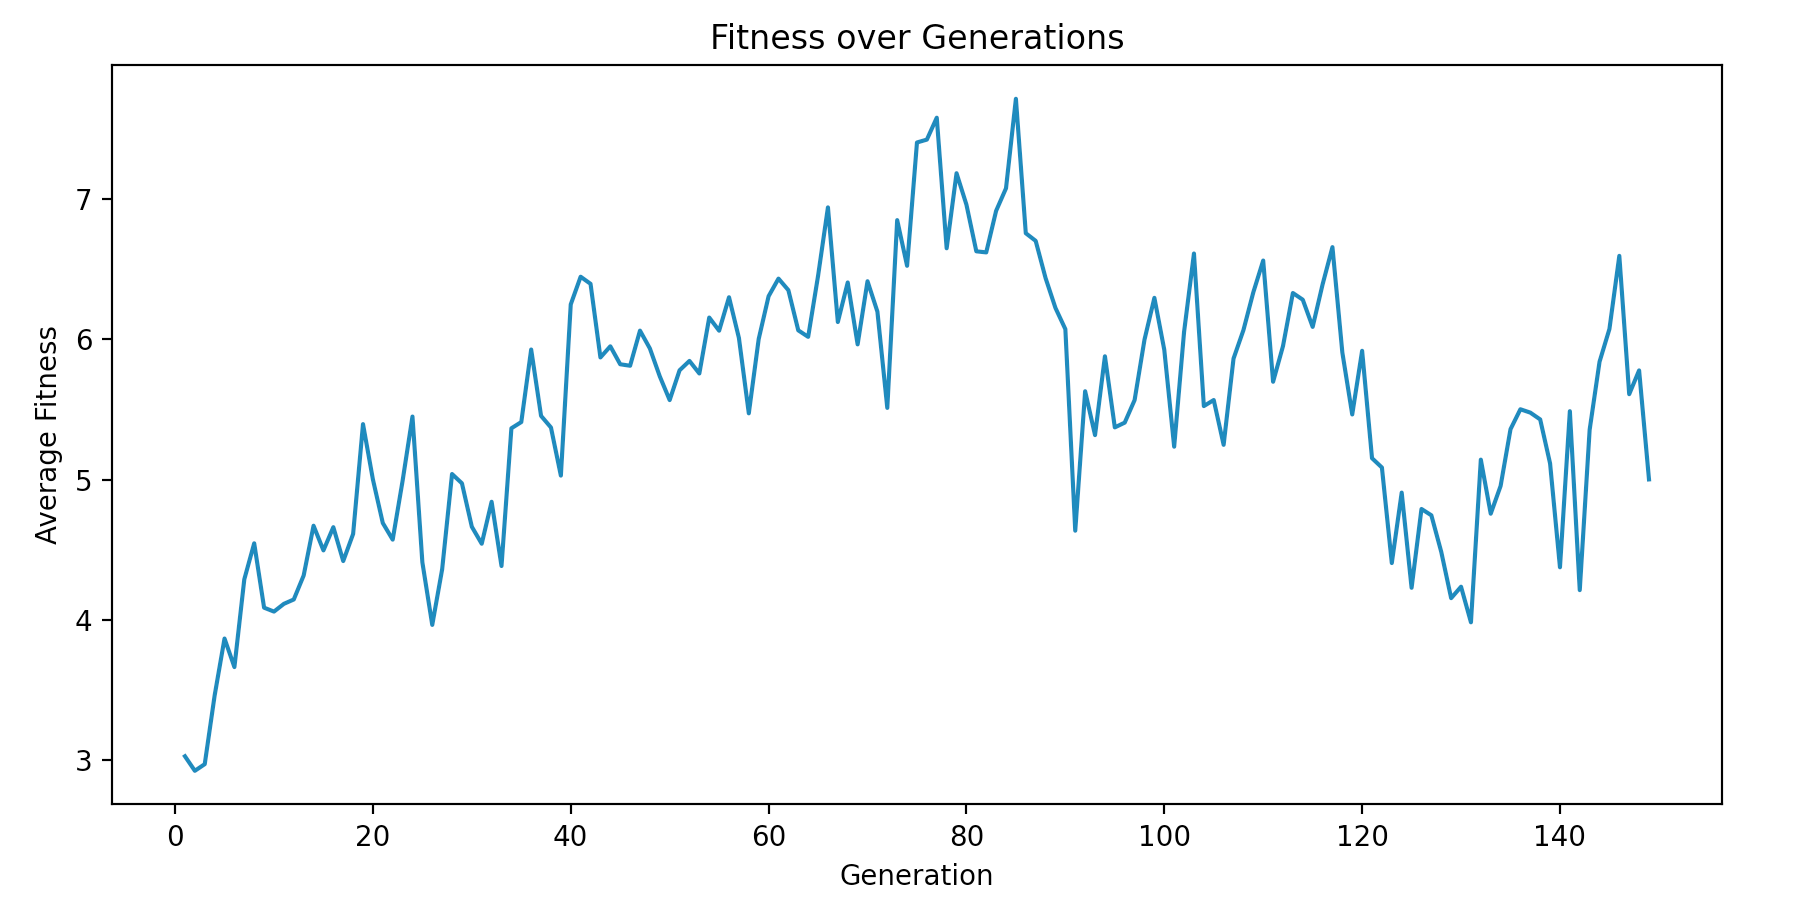
\includegraphics[width=0.5\textwidth]{figures/fitnessGraph_pureElitism.png}
\caption{Elitist method of breeding, and uniform crossover}
\end{figure}

\begin{figure}[h]
\centering
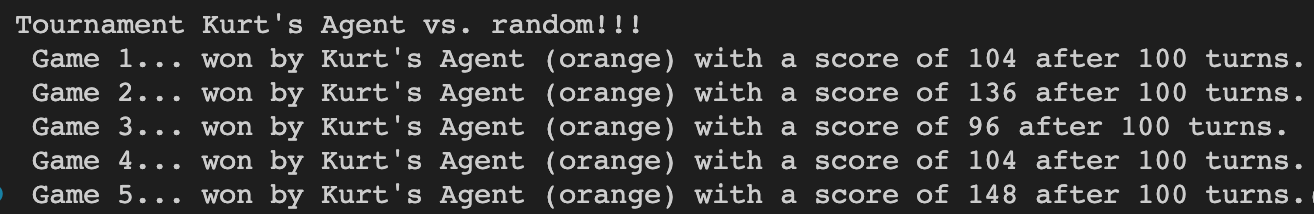
\includegraphics[width=0.5\textwidth]{figures/PureElitismResults.png}
\caption{Elitism method, uniform crossover results.}
\end{figure}

\begin{figure}[h]
\centering
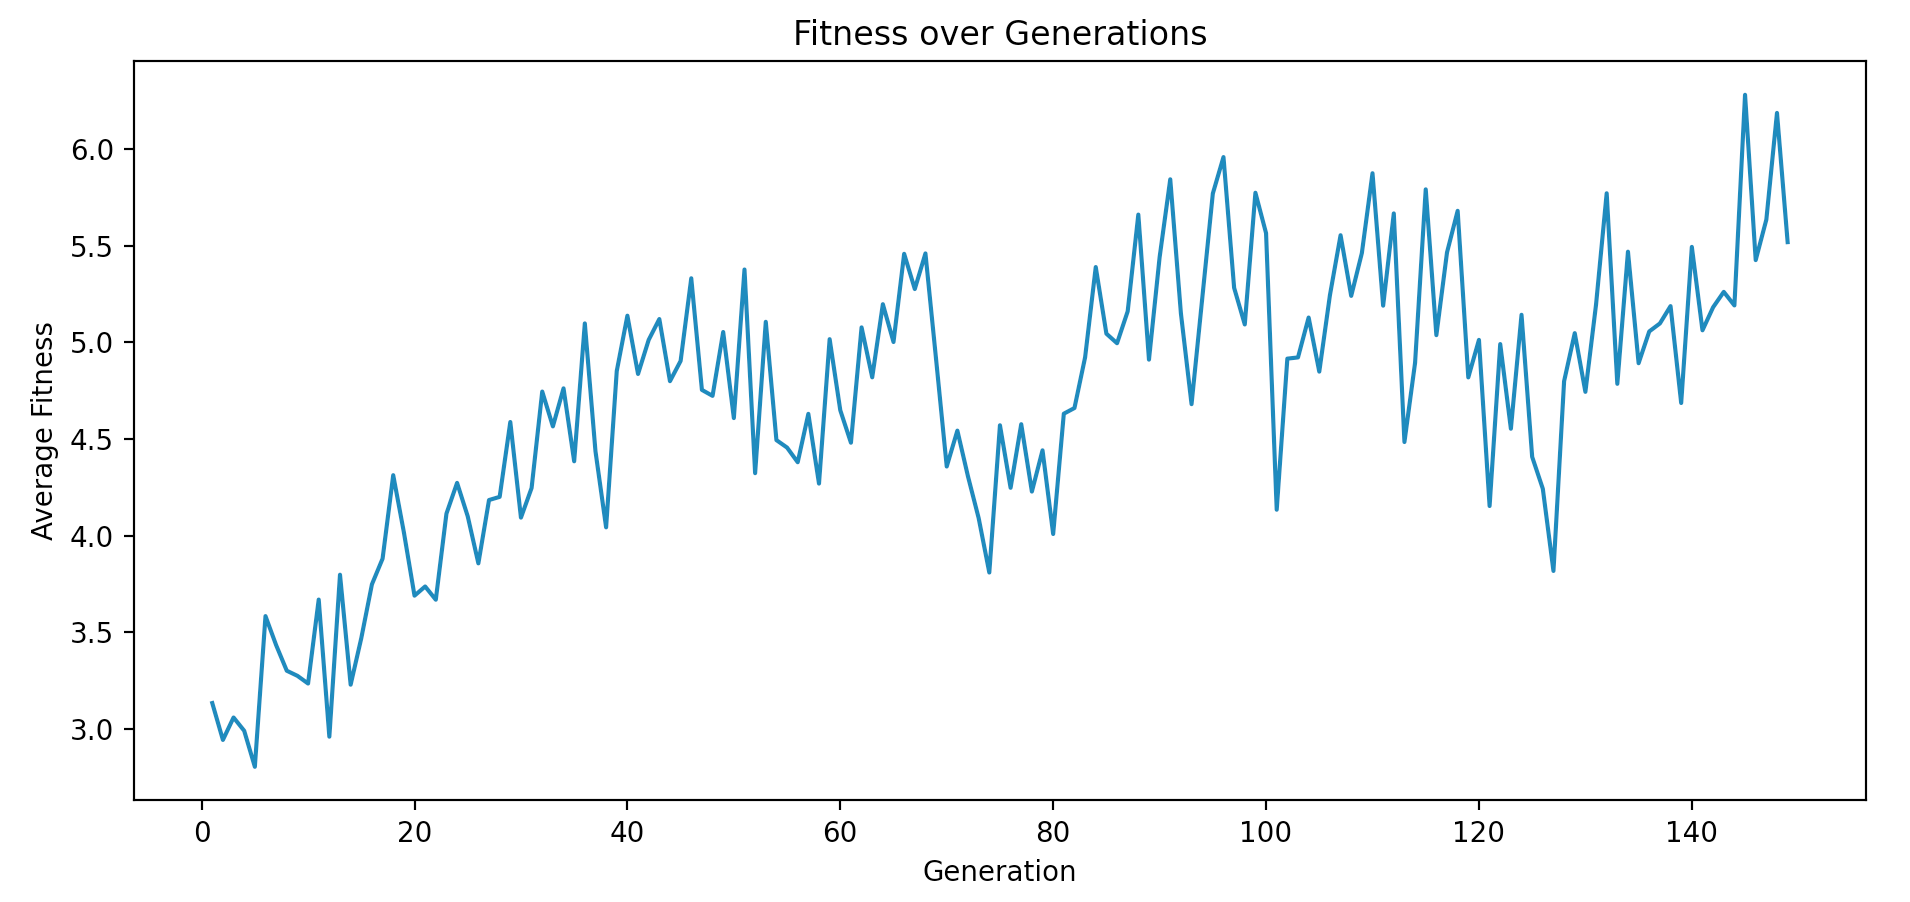
\includegraphics[width=0.4\textwidth]{figures/fitnessGraph_Tournament.png}
\caption{Tournament method of breeding, and 1-point crossover}
\end{figure}

\begin{figure}[h]
\centering
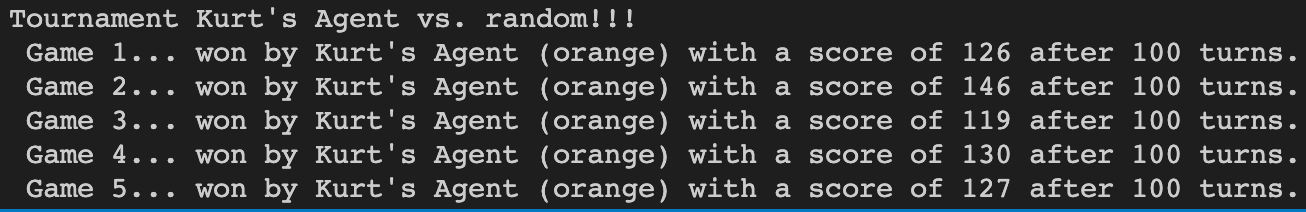
\includegraphics[width=0.4\textwidth]{figures/TournamentResults.png}
\caption{Tournament method, 1-point crossover results.}
\end{figure}

What is interesting in this testing, is that I expected the elitism breeding to be much more effective than the tournament breeding, but they both end up with similar fitnesses, with the tournament breeding fitness continuing to climb, and the elitism breeding fitness falling instead.

The elitism breeding does climb a lot faster than the tournament breeding, but the tournament breeding is more consistent, and the average fitness does not fall towards the end.

More testing could be done to test whether the the 1-point crossover vs uniform crossover is more effective, but since they both use randomness in order to decide whos chromosomes are passed on to children, I assumed it would be a negligible difference.

\subsection{Training}

It is important how the snake agent is trained, as that determines how well the parents do, and what the children inherit.

The method I used to train my snakes was to have them play against themselves for 100 generations in order to teach them to target fruit and avoid themselves and enemies.

Then after they had played 100 generations against themselves, they train 50 generations against the \verb|random_agent|, so they can learn how the agent works, and how to avoid it.

Once they have train for 150 generations, they complete the actual 5 rounds against the \verb|random_agent|, and are scored based on performance.

\section{Conclusion}

Overall, this project taught me a lot about genetic algorithms, and I enjoyed writing the agent and learning about the ways genetic algorithms work.

There is definitely more ways the snakes could be improved, and more testing could be done to show that more generations of snakes provide a significant improvement over previous generations.

A possible way to improve the snake agent would be to take more tiles around the snake into account when deciding a direction for the snake to travel in. This would allow it to predecide its future moves in order to keep itself alive, and collect more food.
\end{document}